% Chapter 1: Number Systems - LaTeX Beamer Slides
% Structured Computer Architecture: An Order-Based Approach
% Authors: John Glossner and Gheorghe M. Ştefan

\documentclass[aspectratio=169,11pt]{beamer}

% Theme and color scheme (simple, print-friendly)
\usetheme{default}
\usecolortheme{default}

% Simple color scheme for printing
\definecolor{titlecolor}{RGB}{0,0,0}
\definecolor{accentcolor}{RGB}{0,0,139}
\definecolor{textcolor}{RGB}{0,0,0}

% Set colors
\setbeamercolor{title}{fg=titlecolor}
\setbeamercolor{frametitle}{fg=titlecolor}
\setbeamercolor{structure}{fg=accentcolor}
\setbeamercolor{normal text}{fg=textcolor}

% Remove navigation symbols
\setbeamertemplate{navigation symbols}{}

% Simple footline
\setbeamertemplate{footline}[frame number]

% Packages
\usepackage{amsmath}
\usepackage{amsfonts}
\usepackage{amssymb}
\usepackage{graphicx}
\usepackage{tikz}
\usepackage{booktabs}
\usepackage{array}
\usepackage{listings}
\usepackage{xcolor}

% Set graphics path for images (relative to slides directory)
\graphicspath{{../Images/}}

% Title information
\title[Part 1: Number Systems]{Structured Computer Architecture}
\subtitle{An Order-Based Approach}
\author{John Glossner and Gheorghe M. Ştefan}
%\institute{Based on the textbook}
\date{\today}

% Custom commands
\newcommand{\concept}[1]{\textbf{\color{accentcolor}#1}}
\newcommand{\defterm}[1]{\textit{#1}}

\begin{document}

%******************************
% Title Slide
%*******************************
\begin{frame}
\titlepage
\end{frame}

%******************************
% Part I Slides (7 chapters)
%*******************************
\part{Number Systems and Representations}

\begin{frame}
\begin{center}
{\Huge Part I}\\[0.5cm]
{\Large Number Systems and Representations}\\[0.5cm]
%{\normalsize Foundations of Digital Representation}
\end{center}
\end{frame}

\section{Number Systems, Sets, and Representations}
\begin{frame}{Outline}
\tableofcontents[sections=1]
\end{frame}

% Learning Objectives
\begin{frame}{Learning Objectives}
By the end of this chapter, you will be able to:
\begin{itemize}
\item Understand the historical evolution of number systems
\item Explain the significance of positional notation
\item Perform arithmetic operations in decimal and binary systems
\item Convert numbers between different bases
\item Understand the mathematical foundations of computing
\item Recognize the progression from manual to digital computation
\end{itemize}
\end{frame}

% subsection 1: Introduction
\subsection{A Brief History of Number Systems}

\begin{frame}{Early Development}
\begin{itemize}
\item \concept{Tally Marks}: Earliest form of numerical representation
\begin{itemize}
\item Used by prehistoric humans for counting
\item Simple one-to-one correspondence
\item Limited scalability for large numbers
\end{itemize}
\vspace{0.5cm}
\item \concept{Ancient Civilizations}: Development of more sophisticated systems
\begin{itemize}
\item Egyptian hieroglyphic numerals
\item Babylonian cuneiform numbers
\item Roman numeral system
\end{itemize}
\end{itemize}
\end{frame}

\begin{frame}{Hindu-Arabic Numeral System}
\begin{itemize}
\item \concept{Revolutionary Innovation}: Developed between 500-1200 CE
\begin{itemize}
\item Introduced the concept of zero
\item Fully positional notation system
\item Foundation for modern mathematics
\end{itemize}
\vspace{0.5cm}
\item \concept{Key Features}:
\begin{itemize}
\item Place value system
\item Ten distinct symbols (0-9)
\item Decimal (base-10) representation
\item Efficient for calculation and representation
\end{itemize}
\end{itemize}
\end{frame}

\begin{frame}{Binary Number System}
\begin{itemize}
\item \concept{Historical Context}: First described by Indian mathematician Pingala
\begin{itemize}
\item Used for prosody and poetry analysis
\item Later formalized by Gottfried Leibniz
\item Foundation for digital computing
\end{itemize}
\vspace{0.5cm}
\item \concept{Digital Revolution}: 
\begin{itemize}
\item Only two states: 0 and 1
\item Perfect match for electronic switches
\item Basis for all digital computation
\end{itemize}
\end{itemize}
\end{frame}

% subsection 2: Evolution of Mathematical Sets
\subsection{Evolution of Mathematical Sets}

\begin{frame}{Mathematical Set Development}
\begin{itemize}
\item \concept{Natural Numbers ($\mathbb{N}$)}: $\{1, 2, 3, 4, ...\}$
\begin{itemize}
\item Used for counting objects
\item Foundation of arithmetic
\end{itemize}
\vspace{0.3cm}
\item \concept{Integers ($\mathbb{Z}$)}: $\{..., -2, -1, 0, 1, 2, ...\}$
\begin{itemize}
\item Includes negative numbers
\item Enables subtraction operations
\end{itemize}
\vspace{0.3cm}
\item \concept{Rational Numbers ($\mathbb{Q}$)}: $\{a/b : a,b \in \mathbb{Z}, b \neq 0\}$
\begin{itemize}
\item Fractions and ratios
\item Extensively studied by Greeks
\end{itemize}
\end{itemize}
\end{frame}

\begin{frame}{Advanced Number Systems}
\begin{itemize}
\item \concept{Real Numbers ($\mathbb{R}$)}:
\begin{itemize}
\item Include irrational numbers
\item Continuous number line
\item Essential for geometry and calculus
\end{itemize}
\vspace{0.5cm}
\item \concept{Complex Numbers ($\mathbb{C}$)}:
\begin{itemize}
\item Form: $a + bi$ where $i = \sqrt{-1}$
\item Emerged in 16th century
\item Solutions to polynomial equations
\item Applications in engineering and physics
\end{itemize}
\end{itemize}
\end{frame}

% subsection 3: Pre-Computer Number Representations
\subsection{Pre-Computer Number Representations}

\begin{frame}{Manual and Mechanical Systems}
\begin{itemize}
\item \concept{Before Digital Computers}:
\begin{itemize}
\item Numerical representations designed for human use
\item Mechanical calculators and slide rules
\item Emphasis on ease of manual calculation
\end{itemize}
\vspace{0.5cm}
\item \concept{Key Characteristics}:
\begin{itemize}
\item Decimal-based systems
\item Visual and tactile interfaces
\item Limited precision and range
\item Human-readable formats
\end{itemize}
\end{itemize}
\end{frame}

% subsection 4: Decimal Positional Systems
\subsection{Decimal Positional Systems}

\begin{frame}{Positional Notation Principles}
\begin{itemize}
\item \concept{Place Value System}:
\begin{itemize}
\item Each position represents a power of the base
\item Rightmost position: $10^0 = 1$
\item Next position: $10^1 = 10$, then $10^2 = 100$, etc.
\end{itemize}
\vspace{0.5cm}
\item \concept{Example}: Number 1,234
\begin{align}
1234 &= 1 \times 10^3 + 2 \times 10^2 + 3 \times 10^1 + 4 \times 10^0\\
&= 1000 + 200 + 30 + 4
\end{align}
\end{itemize}
\end{frame}

\begin{frame}{Medieval Dominance}
\begin{itemize}
\item \concept{Hindu-Arabic System Adoption}:
\begin{itemize}
\item Became dominant during medieval period
\item Replaced Roman numerals for calculation
\item Enabled complex mathematical operations
\end{itemize}
\vspace{0.5cm}
\item \concept{Advantages over Previous Systems}:
\begin{itemize}
\item Compact representation
\item Efficient arithmetic algorithms
\item Scalable to any size number
\item Universal adoption across cultures
\end{itemize}
\end{itemize}
\end{frame}

% subsection 5: Complement Systems
\subsection{10's Complement for Subtraction}

\begin{frame}{Complement Arithmetic}
\begin{itemize}
\item \concept{Historical Context}:
\begin{itemize}
\item Predates computer era
\item Used in mechanical calculators
\item Simplifies subtraction operations
\end{itemize}
\vspace{0.5cm}
\item \concept{10's Complement Method}:
\begin{itemize}
\item Convert subtraction to addition
\item Useful for mechanical computation
\item Foundation for modern computer arithmetic
\end{itemize}
\end{itemize}
\end{frame}

\begin{frame}{10's Complement Example}
\concept{Example}: Calculate $456 - 123$ using 10's complement

\vspace{0.3cm}
\begin{enumerate}
\item Find 10's complement of 123:
\begin{itemize}
\item 9's complement: $999 - 123 = 876$
\item 10's complement: $876 + 1 = 877$
\end{itemize}

\item Add: $456 + 877 = 1333$

\item Remove leading 1: $333$

\item Result: $456 - 123 = 333$ ✓
\end{enumerate}
\end{frame}

% subsection 6: Logarithmic Representations
\subsection{Logarithmic Representations}

\begin{frame}{John Napier's Innovation}
\begin{itemize}
\item \concept{Early 17th Century Development}:
\begin{itemize}
\item John Napier introduced logarithms
\item Enabled multiplication through addition
\item Revolutionary for complex calculations
\end{itemize}
\vspace{0.5cm}
\item \concept{Key Principle}:
\begin{align}
\log(a \times b) = \log(a) + \log(b)
\end{align}
\item \concept{Applications}:
\begin{itemize}
\item Slide rules for engineering
\item Astronomical calculations
\item Navigation and surveying
\end{itemize}
\end{itemize}
\end{frame}

% subsection 7: Number Representations in Computing
\subsection{Number Representations in Computing}

\begin{frame}{Transition to Digital Systems}
\begin{itemize}
\item \concept{Digital Revolution Requirements}:
\begin{itemize}
\item New numerical representations needed
\item Tailored for electronic constraints
\item Optimized for digital processing
\end{itemize}
\vspace{0.5cm}
\item \concept{Key Considerations}:
\begin{itemize}
\item Binary representation (0s and 1s)
\item Fixed-width formats
\item Efficient arithmetic operations
\item Error detection and correction
\end{itemize}
\end{itemize}
\end{frame}

% subsection 8: Binary and Two's Complement
\subsection{Binary and Two's Complement}

\begin{frame}{Binary Number System}
\begin{itemize}
\item \concept{Fundamental Principle}:
\begin{itemize}
\item Base-2 positional system
\item Only two digits: 0 and 1
\item Each position represents power of 2
\end{itemize}
\vspace{0.5cm}
\item \concept{Example}: Binary 1101₂ to Decimal
\begin{align}
1101_2 &= 1 \times 2^3 + 1 \times 2^2 + 0 \times 2^1 + 1 \times 2^0\\
&= 8 + 4 + 0 + 1 = 13_{10}
\end{align}
\end{itemize}
\end{frame}

\begin{frame}{Binary Addition Example}
\begin{columns}
\begin{column}{0.5\textwidth}
\concept{Binary Addition Rules}:
\begin{align}
0 + 0 &= 0\\
0 + 1 &= 1\\
1 + 0 &= 1\\
1 + 1 &= 10_2 \text{ (carry 1)}
\end{align}
\end{column}
\begin{column}{0.5\textwidth}
\concept{Example}: $1011_2 + 1101_2$
\begin{center}
\begin{tabular}{r}
  1011 \\
+ 1101 \\
\hline
 11000 \\
\end{tabular}
\end{center}
Verification: $11 + 13 = 24 = 11000_2$ ✓
\end{column}
\end{columns}
\end{frame}

\begin{frame}{Two's Complement System}
\begin{itemize}
\item \concept{Signed Binary Representation}:
\begin{itemize}
\item Standard for representing negative numbers
\item Simplifies arithmetic operations
\item No separate subtraction circuitry needed
\end{itemize}
\vspace{0.5cm}
\item \concept{Two's Complement Process}:
\begin{enumerate}
\item Invert all bits (one's complement)
\item Add 1 to the result
\end{enumerate}
\vspace{0.3cm}
\item \concept{Example}: -5 in 4-bit two's complement
\begin{itemize}
\item +5: 0101
\item Invert: 1010
\item Add 1: 1011 = -5
\end{itemize}
\end{itemize}
\end{frame}

\begin{frame}{Two's Complement Range}
\begin{itemize}
\item \concept{n-bit Two's Complement Range}:
\begin{itemize}
\item Range: $-2^{n-1}$ to $2^{n-1}-1$
\item Most significant bit is sign bit
\item Asymmetric range (one more negative than positive)
\end{itemize}
\end{itemize}

\vspace{0.5cm}
\begin{center}
\begin{tabular}{|c|c|c|}
\hline
\textbf{Bits} & \textbf{Range} & \textbf{Example} \\
\hline
4 & -8 to +7 & 1000 = -8, 0111 = +7 \\
8 & -128 to +127 & 10000000 = -128 \\
16 & -32,768 to +32,767 & Standard short int \\
32 & $-2^{31}$ to $2^{31}-1$ & Standard int \\
\hline
\end{tabular}
\end{center}
\end{frame}

% subsection 9: Advanced Representations
\subsection{Excess-k and Other Representations}

\begin{frame}{Excess-k (Biased) Representation}
\begin{itemize}
\item \concept{Biased Number System}:
\begin{itemize}
\item Add a bias (k) to the actual value
\item Useful for floating-point exponents
\item Simplifies comparison operations
\end{itemize}
\vspace{0.5cm}
\item \concept{Example}: Excess-127 (8-bit)
\begin{itemize}
\item Bias = 127
\item Range: -127 to +128
\item Stored value = Actual value + 127
\item Zero is represented as 127
\end{itemize}
\end{itemize}

\vspace{0.3cm}
\begin{center}
\begin{tabular}{|c|c|c|}
\hline
\textbf{Actual Value} & \textbf{Stored Value} & \textbf{Binary} \\
\hline
-127 & 0 & 00000000 \\
-1 & 126 & 01111110 \\
0 & 127 & 01111111 \\
+1 & 128 & 10000000 \\
+128 & 255 & 11111111 \\
\hline
\end{tabular}
\end{center}
\end{frame}

% subsection 10: Fixed-Point Arithmetic
\subsection{Fixed-Point Arithmetic}

\begin{frame}{Fixed-Point Number System}
\begin{itemize}
\item \concept{Practical Solution}:
\begin{itemize}
\item For embedded systems and early computers
\item Limited hardware complexity
\item Predictable precision
\end{itemize}
\vspace{0.5cm}
\item \concept{Format}: $s.f$ (sign.fractional)
\begin{itemize}
\item Fixed decimal point position
\item Integer and fractional parts
\item Example: 8.8 format (8 integer, 8 fractional bits)
\end{itemize}
\vspace{0.3cm}
\item \concept{Advantages}:
\begin{itemize}
\item Simple arithmetic operations
\item Predictable range and precision
\item Lower hardware cost
\end{itemize}
\end{itemize}
\end{frame}

\begin{frame}{Fixed-Point Example}
\concept{Example}: 16-bit fixed-point with 8.8 format

\vspace{0.3cm}
\begin{itemize}
\item \concept{Representation}: IIIIIIII.FFFFFFFF
\item \concept{Range}: -128.0 to +127.99609375
\item \concept{Resolution}: $2^{-8} = 0.00390625$
\end{itemize}

\vspace{0.5cm}
\concept{Examples}:
\begin{center}
\begin{tabular}{|c|c|c|}
\hline
\textbf{Decimal} & \textbf{Binary (8.8)} & \textbf{Hex} \\
\hline
12.25 & 00001100.01000000 & 0C40 \\
-5.5 & 11111010.10000000 & FA80 \\
0.75 & 00000000.11000000 & 00C0 \\
\hline
\end{tabular}
\end{center}
\end{frame}

% subsection 11: Floating-Point Systems
\subsection{Floating-Point Systems}

\begin{frame}{Dynamic Range Solution}
\begin{itemize}
\item \concept{Motivation}:
\begin{itemize}
\item Need for wide dynamic range
\item Scientific and engineering applications
\item Automatic scaling of numbers
\end{itemize}
\vspace{0.5cm}
\item \concept{IEEE 754 Standard}:
\begin{itemize}
\item Sign bit (1 bit)
\item Exponent (8 bits for single precision)
\item Mantissa/Significand (23 bits for single precision)
\end{itemize}
\vspace{0.3cm}
\item \concept{Format}: $(-1)^s \times 1.M \times 2^{E-127}$
\end{itemize}
\end{frame}

\begin{frame}{IEEE 754 Single Precision Format}
\begin{center}
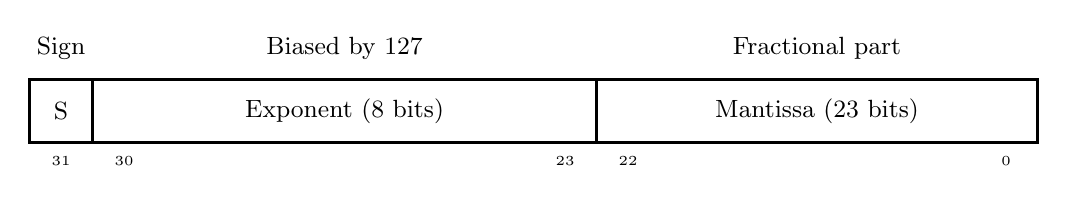
\begin{tikzpicture}[scale=0.8]
% Draw the bit fields
\draw[thick] (0,0) rectangle (1,1);
\draw[thick] (1,0) rectangle (9,1);
\draw[thick] (9,0) rectangle (16,1);

% Labels
\node at (0.5,0.5) {\small S};
\node at (5,0.5) {\small Exponent (8 bits)};
\node at (12.5,0.5) {\small Mantissa (23 bits)};

% Bit numbers
\node at (0.5,-0.3) {\tiny 31};
\node at (1.5,-0.3) {\tiny 30};
\node at (8.5,-0.3) {\tiny 23};
\node at (9.5,-0.3) {\tiny 22};
\node at (15.5,-0.3) {\tiny 0};

% Field descriptions
\node at (0.5,1.5) {\small Sign};
\node at (5,1.5) {\small Biased by 127};
\node at (12.5,1.5) {\small Fractional part};
\end{tikzpicture}
\end{center}

\vspace{0.5cm}
\concept{Key Properties}:
\begin{itemize}
\item \textbf{Range}: $\pm 1.18 \times 10^{-38}$ to $\pm 3.40 \times 10^{38}$
\item \textbf{Precision}: About 7 decimal digits
\item \textbf{Special values}: $\pm 0$, $\pm \infty$, NaN
\end{itemize}
\end{frame}

\begin{frame}{Floating-Point Example}
\concept{Example}: Represent 12.375 in IEEE 754 single precision

\vspace{0.3cm}
\begin{enumerate}
\item Convert to binary: $12.375 = 1100.011_2$
\item Normalize: $1.100011 \times 2^3$
\item Sign bit: 0 (positive)
\item Exponent: $3 + 127 = 130 = 10000010_2$
\item Mantissa: $100011000000000000000_2$ (23 bits)
\end{enumerate}

\vspace{0.3cm}
\concept{Result}: 
\begin{center}
\begin{tabular}{|c|c|c|}
\hline
\textbf{S} & \textbf{Exponent} & \textbf{Mantissa} \\
\hline
0 & 10000010 & 10001100000000000000000 \\
\hline
\end{tabular}
\end{center}

\concept{Verification}: $(-1)^0 \times 1.100011_2 \times 2^{130-127} = 1.100011_2 \times 2^3 = 12.375$ ✓
\end{frame}

% subsection 12: Binary Coded Decimal
\subsection{Binary Coded Decimal (BCD)}

\begin{frame}{BCD Representation}
\begin{itemize}
\item \concept{Hybrid System}:
\begin{itemize}
\item Represents decimal digits in binary
\item Each decimal digit uses 4 bits
\item Maintains decimal semantics
\end{itemize}
\vspace{0.5cm}
\item \concept{Example}: 1234 in BCD
\begin{align}
1234_{10} &= 0001\ 0010\ 0011\ 0100_{BCD}\\
&\neq 10011010010_2 \text{ (pure binary)}
\end{align}
\vspace{0.3cm}
\item \concept{Applications}:
\begin{itemize}
\item Financial calculations (no rounding errors)
\item Display systems (7-segment displays)
\item Decimal arithmetic preservation
\end{itemize}
\end{itemize}
\end{frame}

\begin{frame}{BCD vs. Binary Comparison}
\begin{center}
\begin{tabular}{|c|c|c|}
\hline
\textbf{Decimal} & \textbf{BCD} & \textbf{Pure Binary} \\
\hline
0 & 0000 & 0000 \\
1 & 0001 & 0001 \\
2 & 0010 & 0010 \\
9 & 1001 & 1001 \\
10 & 0001 0000 & 1010 \\
15 & 0001 0101 & 1111 \\
99 & 1001 1001 & 1100011 \\
255 & 0010 0101 0101 & 11111111 \\
\hline
\end{tabular}
\end{center}

\vspace{0.3cm}
\concept{Trade-offs}:
\begin{itemize}
\item \textbf{BCD}: Exact decimal representation, easier decimal I/O
\item \textbf{Binary}: More compact, faster arithmetic
\end{itemize}
\end{frame}

% Summary
\subsection{Chapter Summary}

\begin{frame}{Key Takeaways}
\begin{itemize}
\item \concept{Historical Evolution}:
\begin{itemize}
\item From tally marks to sophisticated digital systems
\item Each system solved specific computational needs
\item Positional notation was revolutionary
\end{itemize}
\vspace{0.3cm}
\item \concept{Mathematical Foundations}:
\begin{itemize}
\item Number sets: $\mathbb{N} \subset \mathbb{Z} \subset \mathbb{Q} \subset \mathbb{R} \subset \mathbb{C}$
\item Positional notation principles
\item Complement arithmetic for subtraction
\end{itemize}
\vspace{0.3cm}
\item \concept{Digital Computing Requirements}:
\begin{itemize}
\item Binary representation for electronic systems
\item Multiple formats for different applications
\item Trade-offs between range, precision, and complexity
\end{itemize}
\end{itemize}
\end{frame}

\begin{frame}{Modern Applications}
\begin{itemize}
\item \concept{Computer Architecture Impact}:
\begin{itemize}
\item All digital systems use these principles
\item Hardware design based on number representations
\item Software algorithms optimized for binary operations
\end{itemize}
\vspace{0.3cm}
\item \concept{Representation Trade-offs}:
\begin{itemize}
\item \textbf{Fixed-point}: Simple, predictable, limited range
\item \textbf{Floating-point}: Wide range, complex, IEEE standard
\item \textbf{BCD}: Exact decimal, larger storage requirement
\item \textbf{Two's complement}: Efficient signed arithmetic
\end{itemize}
\vspace{0.3cm}
\item \concept{Future Considerations}:
\begin{itemize}
\item Quantum computing representations
\item Approximate computing systems
\item Energy-efficient number formats
\end{itemize}
\end{itemize}
\end{frame}

% Questions slide
\begin{frame}{Questions and Discussion}
\begin{center}
\Large
Questions?

\vspace{1cm}

\normalsize
\textbf{Discussion Topics:}
\begin{itemize}
\item Why did binary become the standard for digital computers?
\item What are the advantages of two's complement over other signed representations?
\item When would you choose fixed-point over floating-point arithmetic?
\item How do number representation choices affect computer architecture?
\end{itemize}

\vspace{0.5cm}
\textbf{Next:} Chapter 2 - Formal Notation and Mathematical Foundations
\end{center}
\end{frame}




%******************************
% Part II Slides
%*******************************
\part{From Gates to Processors}

\begin{frame}
\begin{center}
{\Huge Part II}\\[0.5cm]
{\Large From Gates to Processors}\\[0.5cm]
%{\normalsize Foundations of Digital Representation}
\end{center}
\end{frame}

%***************************************
% Chapter 02_08: Combinational Circuits
%***************************************
\section{Combinational Circuits: No-Loop, Zero-Order Systems (0-OS)}

\begin{frame}
\begin{center}
{\Huge Chapter 8: Combinational Circuits}\\[0.5cm]
{\Large No-Loop, Zero-Order Systems (0-OS)}\\[0.5cm]
%{\normalsize Foundations of Digital Representation}
\end{center}
\end{frame}

\begin{frame}{Outline}
\tableofcontents[sections=2]
\end{frame}
\input{Latex/slides/02_08_slides}

%***************************************
% Chapter 02_09: Memory Circuits
%***************************************
\section{Memory Circuits: One-Loop, First-Order Systems (1-OS)}

\begin{frame}
\begin{center}
{\Huge Chapter 9: Memory Circuits}\\[0.5cm]
{\Large One-Loop, First-Order Systems (1-OS)}\\[0.5cm]
%{\normalsize Foundations of Digital Representation}
\end{center}
\end{frame}

\begin{frame}{Outline}
\tableofcontents[sections=3]
\end{frame}
\input{Latex/slides/02_09_slides}

%***************************************
% Chapter 02_10: Automata
%***************************************
\section{Automata: Two-Loop, Second-Order Systems (2-OS)}

\begin{frame}
\begin{center}
{\Huge Chapter 10: Automata}\\[0.5cm]
{\Large Two-Loop, Second-Order Systems (2-OS)}\\[0.5cm]
%{\normalsize Foundations of Digital Representation}
\end{center}
\end{frame}

\begin{frame}{Outline}
\tableofcontents[sections=4]
\end{frame}
\input{Latex/slides/02_10_slides}

%***************************************
% Chapter 02_11: Processors
%***************************************
\section{Processors: Three-Loop, Third-Order Systems (3-OS)}

\begin{frame}
\begin{center}
{\Huge Chapter 11: Processors}\\[0.5cm]
{\Large Three-Loop, Third-Order Systems (3-OS)}\\[0.5cm]
%{\normalsize Foundations of Digital Representation}
\end{center}
\end{frame}

\begin{frame}{Outline}
\tableofcontents[sections=5]
\end{frame}
\input{Latex/slides/02_11_slides}


\end{document}
